%%%%%%%%%%%%%%%%%%%%%%%%%%%%%%%%%%%%%%%%%%%%%%%%%%%%%%%%%%%%%%%%%%%%%%%%%%%%%%%%%%
\begin{frame}[fragile]\frametitle{}
\begin{center}
{\Large Chatbot with Slots Filling}
\end{center}

{\tiny (Ref: https://rasa.com/docs/nlu/0.13.5/quickstart/)}
\end{frame}

%%%%%%%%%%%%%%%%%%%%%%%%%%%%%%%%%%%%%%%%%%%%%%%%%%%%%%%%%%%
 \begin{frame}[fragile]\frametitle{What is Slot Filling?}
\begin{itemize}
\item A query may need more than one enitites to be collected first before firing the API or SQL call.
\item Such requite items can get asked over multiple conversations. These items are called as SLOTS.
\item One slot filling scenario could be:
\begin{itemize}
\item user: ``I want Pizza'' \#missing slots: [size, toppings]
\item bot: ``what size?''
\item user: ``large'' \# size is filled now missing slots: [toppings]
\item bot: ``Which toppings would you like?'' 
\item user: ``Olives'' \# toppings is filled now missing slots: [], ready to book the order!!
\end{itemize}
\item In this example we have 2 interactions with the user and 2 slots to fill.
\end{itemize}

\end{frame}


%%%%%%%%%%%%%%%%%%%%%%%%%%%%%%%%%%%%%%%%%%%%%%%%%%%%%%%%%%%
 \begin{frame}[fragile]\frametitle{Domain file}
\begin{lstlisting}
intents:
    - order_pizza
    - greet

entities:
    - size
    - toppings

slots:
    size:
         type: text
    toppings:
        type: text

\end{lstlisting}
\end{frame}



%%%%%%%%%%%%%%%%%%%%%%%%%%%%%%%%%%%%%%%%%%%%%%%%%%%%%%%%%%%
 \begin{frame}[fragile]\frametitle{Domain file}
\begin{lstlisting}
templates:
    utter_greet:
        - 'Hello, how can I help you?'
        - 'Hi, I am here to help.'
    utter_get_pizza_size:
        - 'What pizza size?'
    utter_get_pizza_toppings:
        - 'What toppings would you like on your pizza?'
actions:
    - utter_greet
    - utter_get_pizza_size
    - utter_get_pizza_toppings
    - actions.ActionOrderPizza
\end{lstlisting}
\end{frame}

%%%%%%%%%%%%%%%%%%%%%%%%%%%%%%%%%%%%%%%%%%%%%%%%%%%%%%%%%%%
 \begin{frame}[fragile]\frametitle{RASA Core: Actions and Stories}
\begin{itemize}
\item Actions are either utterances, which means, the output that we want to send the user, or you can actually create your own class that inherent form Action. 
\item Say: ``actions.ActionOrderPizza'', here again Rasa has a very cool interface, you should inherent from Class Action and add your logic in the derived class according to what you need, here is an example, create the file action.py:
\begin{lstlisting}
from rasa_core.actions import Action

class ActionOrderPizza(Action):
    def name(self):
        return 'action_order_pizza'
    def run(self):
        print('Ordering Pizza is completed! It should be with you soon :)')
        pass
\end{lstlisting}
		
\end{itemize}

\end{frame}

%%%%%%%%%%%%%%%%%%%%%%%%%%%%%%%%%%%%%%%%%%%%%%%%%%%%%%%%%%%
 \begin{frame}[fragile]\frametitle{RASA Core: Actions and Stories}
\begin{itemize}
\item But first let's create a very short and basic flow, and train the dialogue model
\item For the basic flow you can use this file stories.md:
\begin{lstlisting}
* greet
    - utter_greet
* order_pizza
    - utter_get_pizza_size
* order_pizza
    - utter_get_pizza_toppings
* order_pizza
    - action_order_pizza
\end{lstlisting}
		
\end{itemize}

\end{frame}

%%%%%%%%%%%%%%%%%%%%%%%%%%%%%%%%%%%%%%%%%%%%%%%%%%%%%%%%%%%
 \begin{frame}[fragile]\frametitle{Train the Dialog}
\begin{lstlisting}
import logging
from rasa_core.agent import Agent
from rasa_core.domain import Domain
from rasa_core.policies.keras_policy import KerasPolicy
from rasa_core.policies.memoization import MemoizationPolicy

if __name__ == '__main__':
    logging.basicConfig(level='INFO')
    dialog_training_data_file = './data/stories.md'
    path_to_model = './models/dialogue'
    # domain = Domain()
    agent = Agent('chat_domain.yml', policies = [MemoizationPolicy(augmentation_factor=50,max_history=2), KerasPolicy(epochs=500,batch_size=10,validation_split=0.2)])

    agent.persist(path_to_model)
    agent.train(dialog_training_data_file)
\end{lstlisting}
\end{frame}

%%%%%%%%%%%%%%%%%%%%%%%%%%%%%%%%%%%%%%%%%%%%%%%%%%%%%%%%%%%%%%%%%%%%%%%%%%%%%%%%%%
\begin{frame}[fragile]\frametitle{}
\begin{center}
{\Large Full Worklfow: Flight Search Chatbot}
\end{center}

{\tiny (Ref:Build a Flight search chatbot from scratch using RASA - Ashutosh Krishna, Medium)}
\end{frame}

%%%%%%%%%%%%%%%%%%%%%%%%%%%%%%%%%%%%%%%%%%%%%%%%%%%%%%%%%%%
 \begin{frame}[fragile]\frametitle{Introduction}
\begin{itemize}
\item Flight Information using search results from Make My Trip(MMT) flight booking website	
\item Not using APIs but parsing search results.
\item Main idea is to learn how to save source-destination cities and date, to query the flight fares.
\end{itemize}

\end{frame}

%%%%%%%%%%%%%%%%%%%%%%%%%%%%%%%%%%%%%%%%%%%%%%%%%%%%%%%%%%%
 \begin{frame}[fragile]\frametitle{Natural Language Understanding}
 
    \begin{columns}
    \begin{column}[t]{0.5\linewidth}
\begin{itemize}
\item Create a Data file which defines intents
\item Four intents(flight,inform,affirmation,deny)
\item Marked the entities for some of the user inputs such as location and date. (for e.g. [DEL](location) `DEL' is the value while `location is the entity').
\end{itemize}
\end{column}
    \begin{column}[t]{0.5\linewidth}
\begin{center}
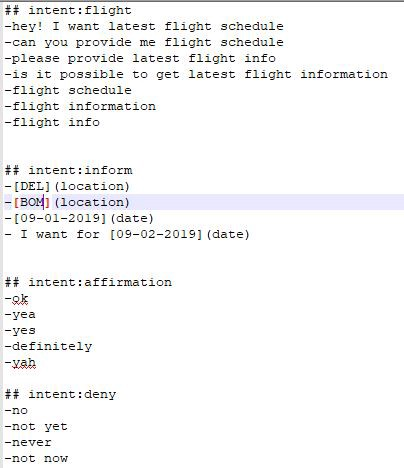
\includegraphics[width=\linewidth,keepaspectratio]{images/mmt1}
\end{center}
\end{column}
\end{columns}
\end{frame}

%%%%%%%%%%%%%%%%%%%%%%%%%%%%%%%%%%%%%%%%%%%%%%%%%%%%%%%%%%%
 \begin{frame}[fragile]\frametitle{Configuration}
 
    \begin{columns}
    \begin{column}[t]{0.5\linewidth}
\begin{itemize}
\item Defines the pipeline. Incoming messages are processed by a sequence of components. These components are executed one after another in a so-called processing pipeline. 
\item There are components for entity extraction, for intent classification, pre-processing, and others. 
\end{itemize}
\end{column}
    \begin{column}[t]{0.5\linewidth}
\begin{center}
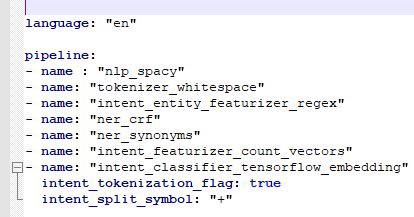
\includegraphics[width=\linewidth,keepaspectratio]{images/mmt2}
\end{center}
\end{column}
\end{columns}
\end{frame}

%%%%%%%%%%%%%%%%%%%%%%%%%%%%%%%%%%%%%%%%%%%%%%%%%%%%%%%%%%%
 \begin{frame}[fragile]\frametitle{Train the NLU Model}
 Train the model with NLU data and config pipelines. The model gets saved inside models/nlu.

\begin{center}
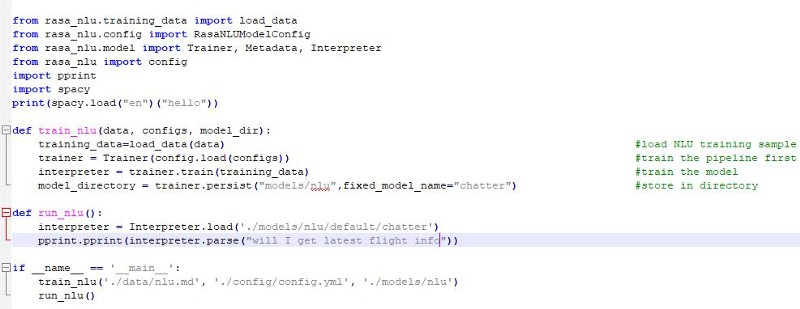
\includegraphics[width=\linewidth,keepaspectratio]{images/mmt3}
\end{center}

\end{frame}

%%%%%%%%%%%%%%%%%%%%%%%%%%%%%%%%%%%%%%%%%%%%%%%%%%%%%%%%%%%
 \begin{frame}[fragile]\frametitle{Evaluate the NLU Model}
Parsed the question (``will I get latest flight info'') and confidence comes out to be 95\% for the intent: flight. That means ,our model is trained well.

\begin{center}
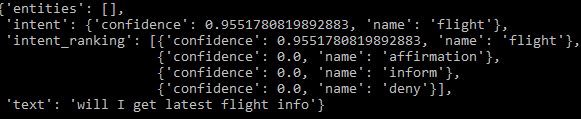
\includegraphics[width=\linewidth,keepaspectratio]{images/mmt4}
\end{center}

\end{frame}

%%%%%%%%%%%%%%%%%%%%%%%%%%%%%%%%%%%%%%%%%%%%%%%%%%%%%%%%%%%
 \begin{frame}[fragile]\frametitle{Domain }
 
    \begin{columns}
    \begin{column}[t]{0.5\linewidth}
\begin{itemize}
\item Defines the universe in which your bot operates. It specifies the intents, entities, slots, and actions your bot should know about. It also includes templates for the things your bot can say. 
\item We get the intents and entities from the NLU model. Slots are the things we want to keep track of during a conversation. 
\item Actions are the things your bot can actually do(such as responding to user, making an external API call, querying a database, setting up slots and many other things). 
\end{itemize}
\end{column}
    \begin{column}[t]{0.5\linewidth}
\begin{center}
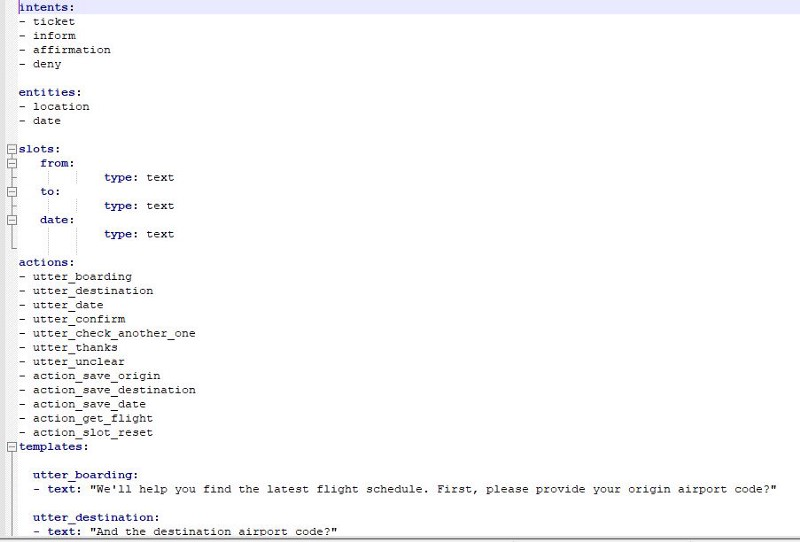
\includegraphics[width=\linewidth,keepaspectratio]{images/mmt5}
\end{center}
\begin{itemize}
\item Utterance templates(utter\_) are messages the bot will send back to the user. utter\_unclear triggers when there is a fallback condition 
\item Curly braces {} fetch slot values to be used in bot utterances.
\end{itemize}
\end{column}
\end{columns}
\end{frame}

%%%%%%%%%%%%%%%%%%%%%%%%%%%%%%%%%%%%%%%%%%%%%%%%%%%%%%%%%%%
 \begin{frame}[fragile]\frametitle{Actions }
 
    \begin{columns}
    \begin{column}[t]{0.5\linewidth}
\begin{itemize}
\item Actions are the things that the bot runs in response to user input. There are some default actions like action\_restart,action\_default\_fallback, action\_listen. 
\item But here we are using custom actions to save slots, connect to MMT website and get flight status.
\item Using BeautifulSoup to do web-scraping
\end{itemize}
\end{column}
    \begin{column}[t]{0.5\linewidth}
\begin{center}
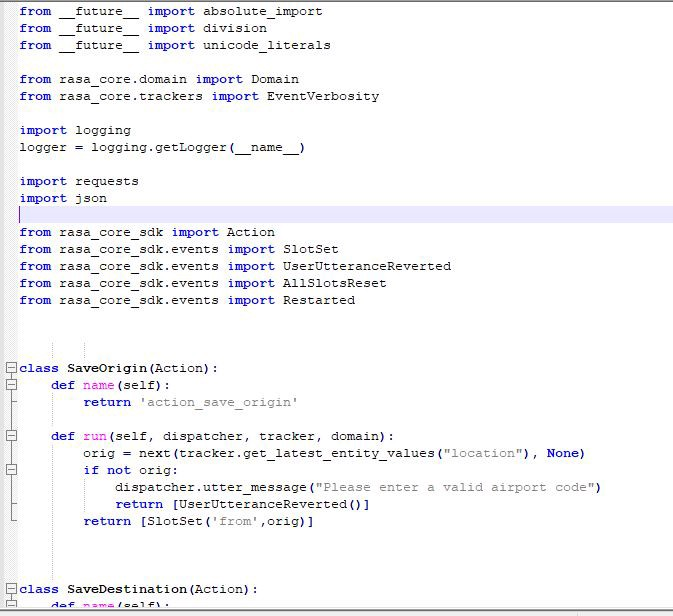
\includegraphics[width=\linewidth,keepaspectratio]{images/mmt6}
\end{center}
\end{column}
\end{columns}
\end{frame}

%%%%%%%%%%%%%%%%%%%%%%%%%%%%%%%%%%%%%%%%%%%%%%%%%%%%%%%%%%%
 \begin{frame}[fragile]\frametitle{Stories }
 
    \begin{columns}
    \begin{column}[t]{0.5\linewidth}
\begin{itemize}
\item Stories tell the model what are the possible flows of conversational dialog
\item Rasa Core works by creating training data from the stories and training a model on that data.
\end{itemize}
\end{column}
    \begin{column}[t]{0.5\linewidth}
\begin{center}
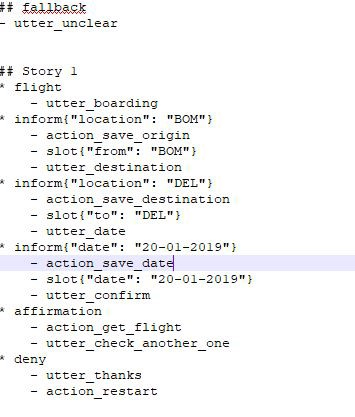
\includegraphics[width=\linewidth,keepaspectratio]{images/mmt7}
\end{center}
\end{column}
\end{columns}
\end{frame}

%%%%%%%%%%%%%%%%%%%%%%%%%%%%%%%%%%%%%%%%%%%%%%%%%%%%%%%%%%%
 \begin{frame}[fragile]\frametitle{Training the Dialog Model}


\begin{center}
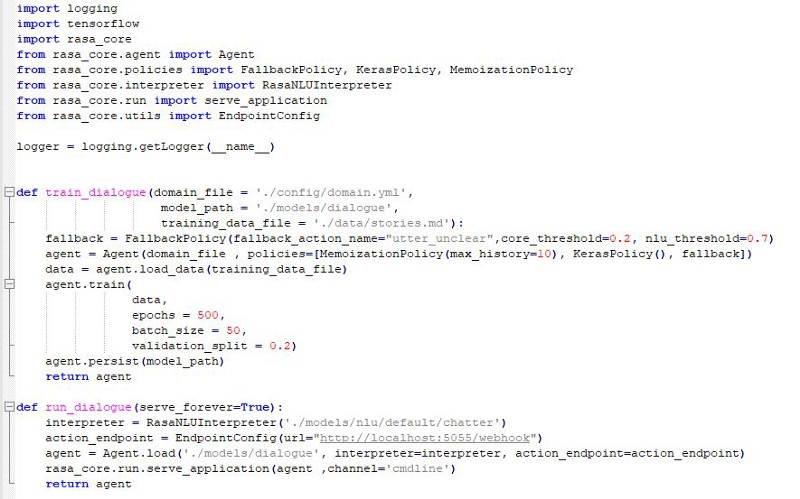
\includegraphics[width=\linewidth,keepaspectratio]{images/mmt8}
\end{center}

\end{frame}

%%%%%%%%%%%%%%%%%%%%%%%%%%%%%%%%%%%%%%%%%%%%%%%%%%%%%%%%%%%
 \begin{frame}[fragile]\frametitle{Run the Bot}

The NLU model and core model is loaded in Agent through which we pass queries and get a response.

\begin{center}
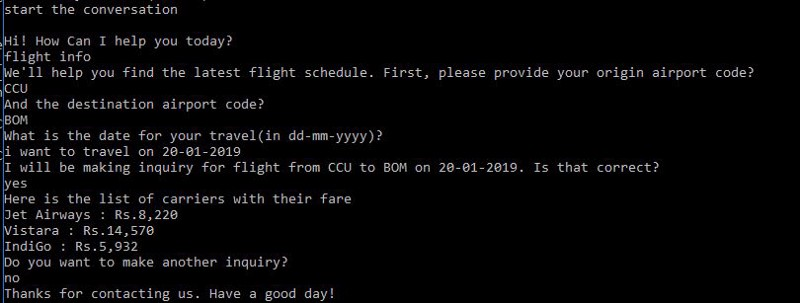
\includegraphics[width=\linewidth,keepaspectratio]{images/mmt9}
\end{center}

\end{frame}

%%%%%%%%%%%%%%%%%%%%%%%%%%%%%%%%%%%%%%%%%%%%%%%%%%%%%%%%%%%
 \begin{frame}[fragile]\frametitle{Next: More Stories with Interactive Learning}
\begin{itemize}
\item In interactive learning mode, you provide feedback to your bot while you talk to it. This is a powerful way to explore what your bot can do, and the easiest way to fix any mistakes it makes. 
\item One advantage of machine learning-based dialogue is that when your bot doesn't know how to do something yet, you can just teach it!
\item Run \lstinline|python -m rasa_core.train-online -d config/domain.yml -s data/stories.md -o models/dialogue -u models/nlu/default/chatter -epochs 250 -endpoints endpoints.yml|
\end{itemize}
\end{frame}